\section{Synthetic Data Studies}

\begin{frame}
  \frametitle{Synthetic Data Studies}
  \begin{figure}
    \centering
    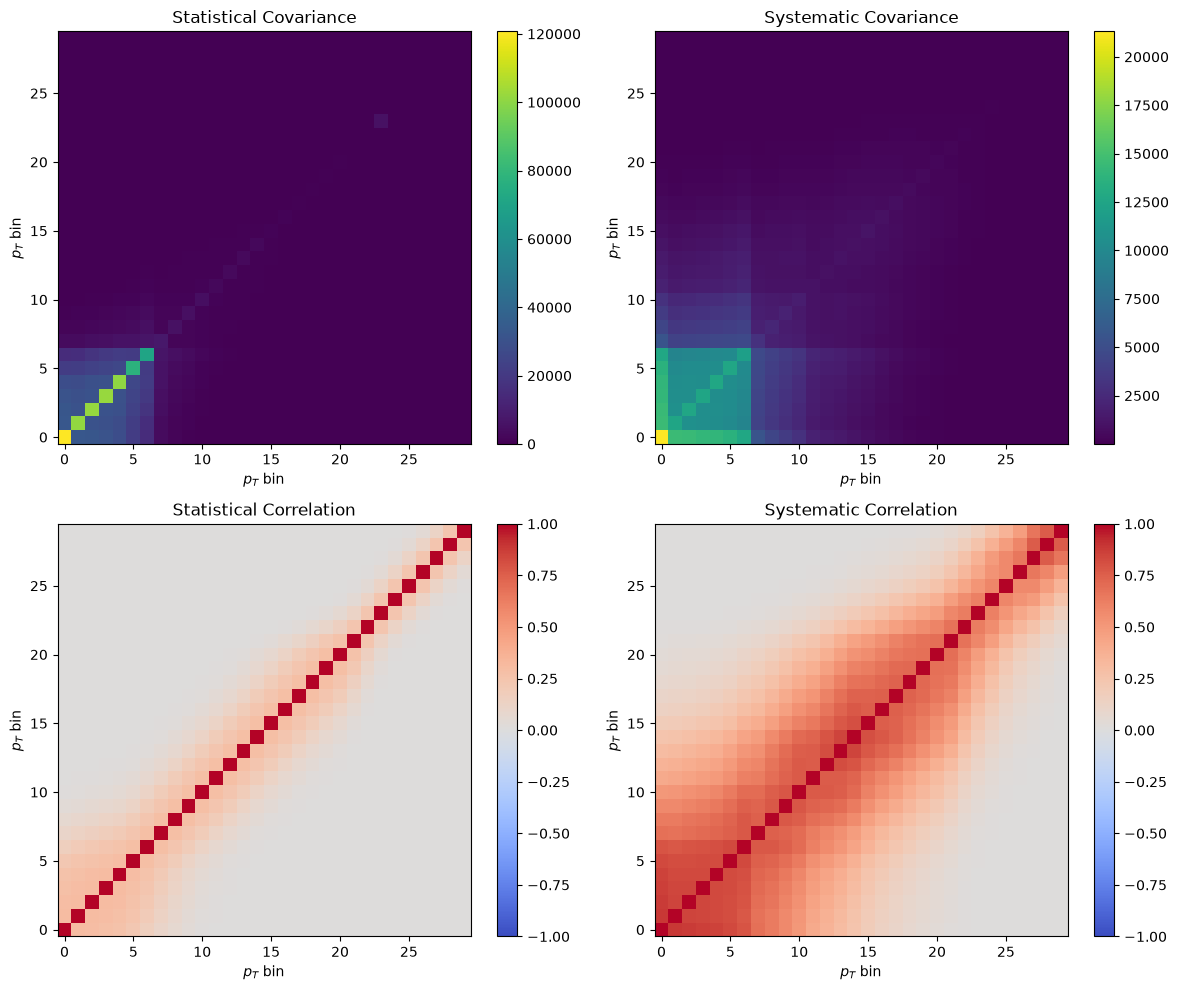
\includegraphics[width=\linewidth,height=0.68\textheight,keepaspectratio]{img/synthetic_v2_covariance_correlation.png}
    \caption{Statistical and systematic covariance used to construct the synthetic data.}
  \end{figure}
\end{frame}

\begin{frame}
  \frametitle{Synthetic Data Studies}
  \begin{figure}
    \centering
    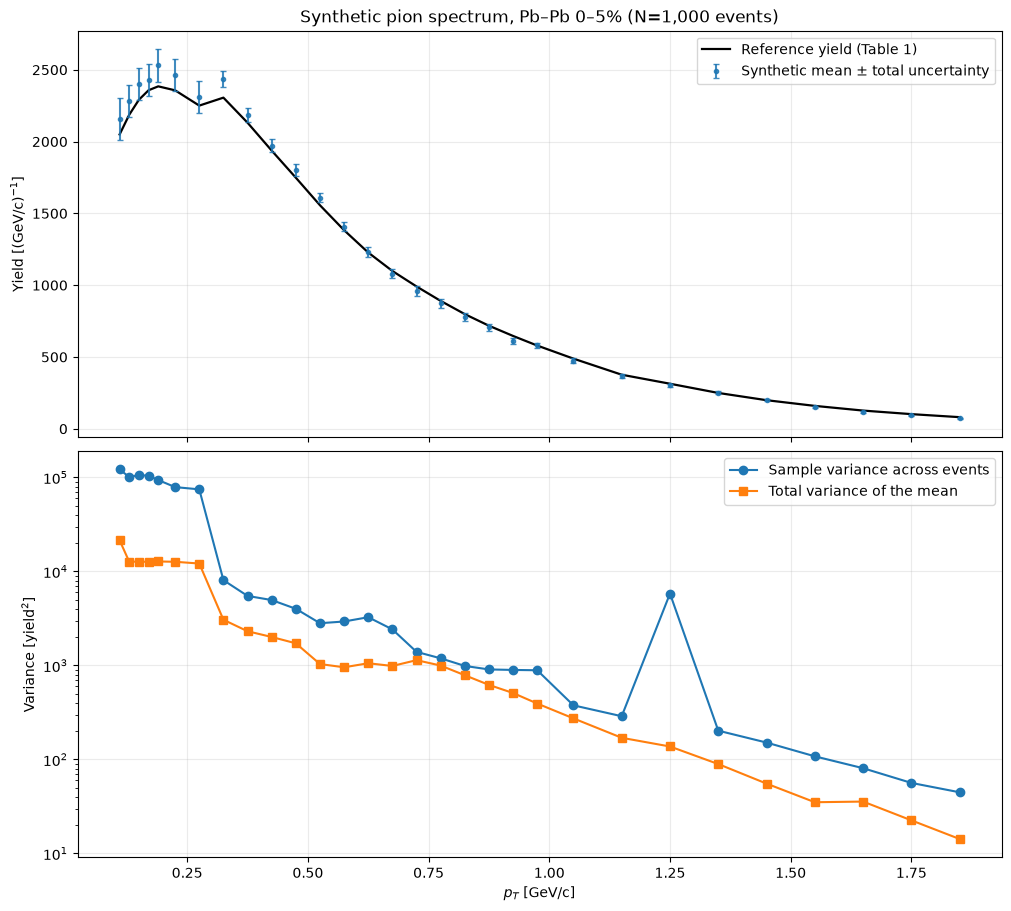
\includegraphics[width=\linewidth,height=0.68\textheight,keepaspectratio]{img/synthetic_v2_spectrum_variances.png}
    \caption{Mean values and variances in each bin of the synthetic data.}
  \end{figure}
\end{frame}

\begin{frame}
  \frametitle{Classical vs Quantum covariance estimation}
  \begin{figure}
    \centering
    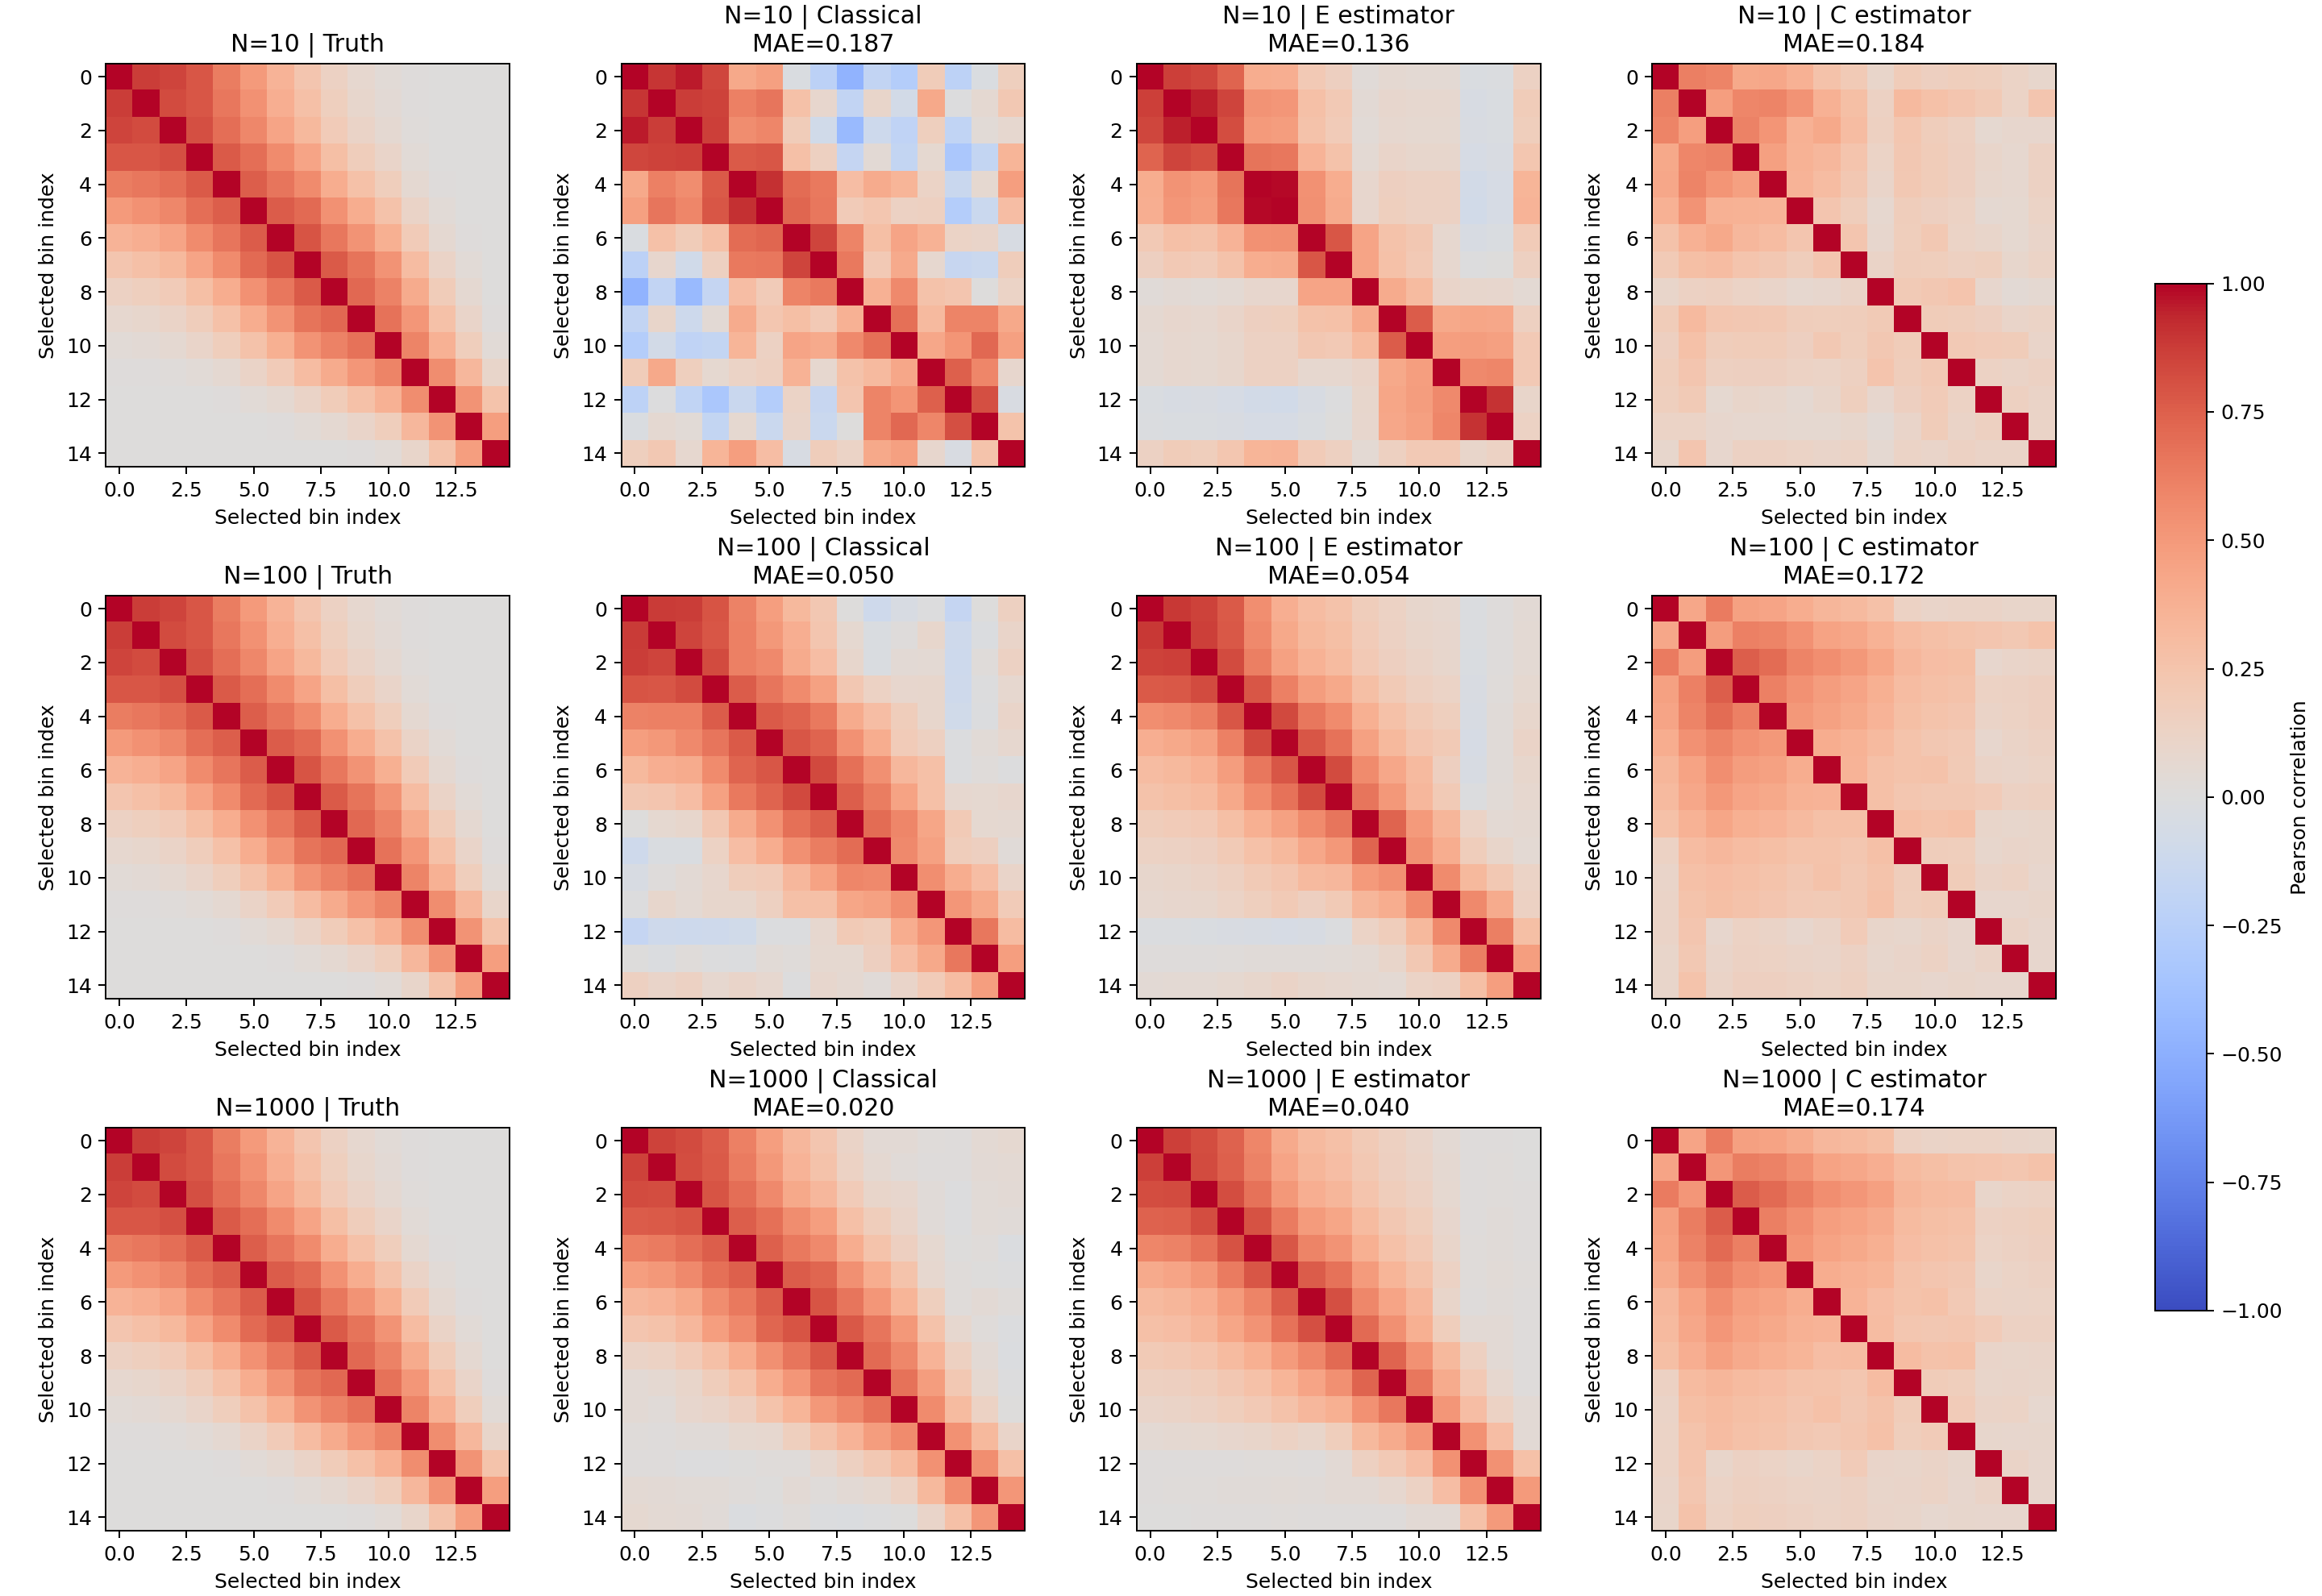
\includegraphics[width=\linewidth,height=0.68\textheight,keepaspectratio]{img/pearson_comparison_N10_100_1000.png}
    \caption{Comparing classical and quantum correlation estimates using 10, 100, and 1000 samples.}
  \end{figure}
\end{frame}
